\documentclass[a4paper,12pt]{report}
\usepackage[utf8]{inputenc}
\usepackage{polski}
\documentclass[a4paper,12pt]{article}
\usepackage[utf8]{inputenc}
\usepackage{graphicx}
\usepackage{float}
\usepackage{hyperref}
\usepackage{array}

\title{Sprawozdanie Megusta+

\newline Projektowanie i programowanie \newline systemów internetowych I 
\newline prowadzący: mgr inż. Krzysztof Rewak
}

\author{Grupa s2PAM2u Andrzej Czabajski, Dominik Kamiński, Jan Łabaj}

\begin{document}

\maketitle

\tableofcontents

\chapter{Wstęp}

W dzisiejszych czasach, kiedy coraz większą wagę przykładamy do zdrowego stylu życia i świadomego odżywiania, niezwykle istotne staje się monitorowanie i ocena spożywanych produktów. Aplikacja \textbf{Megusta} została stworzona z myślą o użytkownikach, którzy chcą aktywnie zarządzać swoją dietą, oceniać produkty spożywcze i podejmować lepsze decyzje żywieniowe.

\textbf{Megusta} to innowacyjne narzędzie, które umożliwia użytkownikom ocenianie produktów spożywczych na podstawie ich własnych preferencji smakowych, wartości odżywczych oraz innych kryteriów.



\begin{figure}[h!]
    \centering
    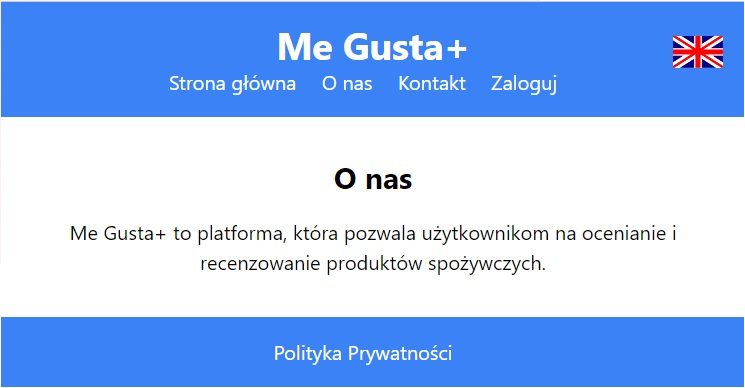
\includegraphics[width=\textwidth]{00logo.jpg}
    
\end{figure}

\chapter{Opis Funkcjonalny Systemu}
Megusta oferuje następujące główne funkcjonalności:
\begin{itemize}
    \item \textbf{Wielojęzyczność}: Strona obsługuje dwa języki polski i angielski poprzez wykrycie preferencji językowych przeglądarki użytkownika i ustawiając odpowiednie ciasteczko.
    
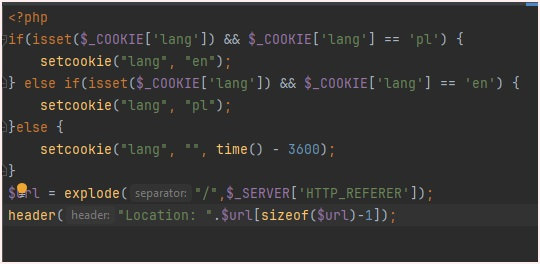
\includegraphics[width=\textwidth]{01A_Lokalizacja.jpg}
    
    \item \textbf{Routing}: System routingu kieruje żądania URL do odpowiednich modułów, umożliwiając dynamiczne generowanie treści.

Routing na tej stronie działa poprzez klasę Router, która zarządza ścieżkami URL i kieruje żądania do odpowiednich modułów w aplikacji. Oto kluczowe elementy działania routingu:

Inicjalizacja:

Kiedy użytkownik odwiedza stronę, index.php tworzy instancję klasy Router, przekazując jej obiekt bazy danych, bieżący URI oraz logger.
Konstruktor klasy Router ustawia globalną zmienną administratora i loguje żądanie użytkownika.
Analiza URL:

Metoda getParameters() rozbija URI na segmenty i usuwa pierwsze dwa elementy, co pozwala na uzyskanie parametrów ścieżki.
Ładowanie Modułu:

Metoda loadModule() tworzy instancję klasy HTMLGenerator i sprawdza, czy istnieje odpowiedni szablon w zależności od języka ustawionego w ciasteczkach.
Jeśli szablon istnieje, ustawia go jako katalog szablonów. Jeśli użytkownik jest administratorem, ustawia szablon panelu administracyjnego.
Generuje i wyświetla stronę za pomocą metody generate() klasy HTMLGenerator.
Sprawdzenie Administratora:

Metoda isAdmin() sprawdza, czy ciasteczko użytkownika zawiera token administratora i zwraca odpowiednią wartość logiczną.
Ustawienie Globalnego Administratora:

Metoda setAdminGlobal() wykonuje zapytanie do bazy danych, aby ustawić token administratora jako globalną zmienną.
Dzięki tym krokom, klasa Router efektywnie zarządza routingiem na stronie, kierując użytkowników do odpowiednich szablonów i modułów na podstawie URL, języka oraz uprawnień użytkownika.

\newpage   

    \item \textbf{Panel Administracyjny}: Umożliwia zarządzanie treścią, która docelowo znajdzie się na stronie. Tylko Administrator może dodawać nowego produkty i opisy.

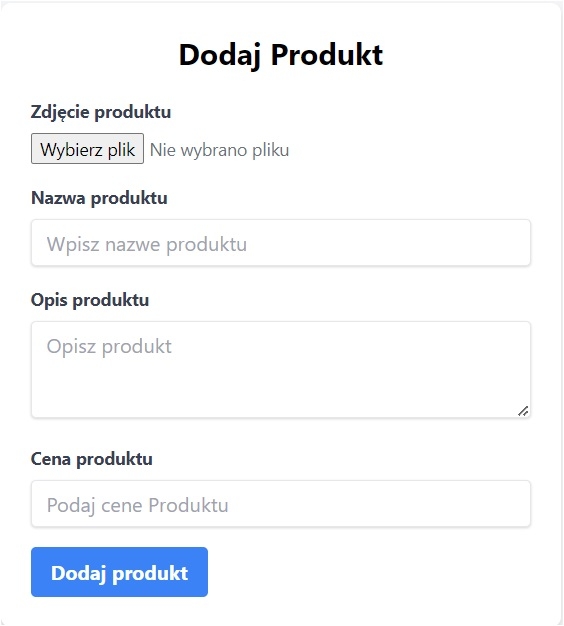
\includegraphics[width=\textwidth]{02Panel.jpg}

\newpage    
    \item \textbf{Logowanie Aktywności}: Logowanie informacji i błędów w celu monitorowania i debugowania aplikacji.

    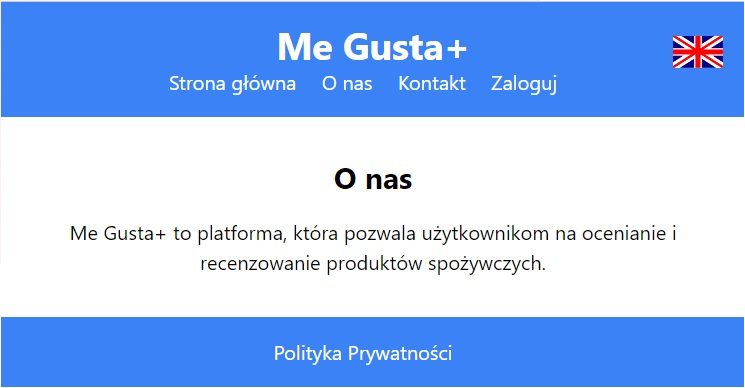
\includegraphics[width=\textwidth]{00logo.jpg}

\newpage  
    
    \item \textbf{Interfejs Użytkownika}: Responsywny interfejs użytkownika stylizowany za pomocą Tailwind CSS, zapewniający estetyczny i spójny wygląd.

    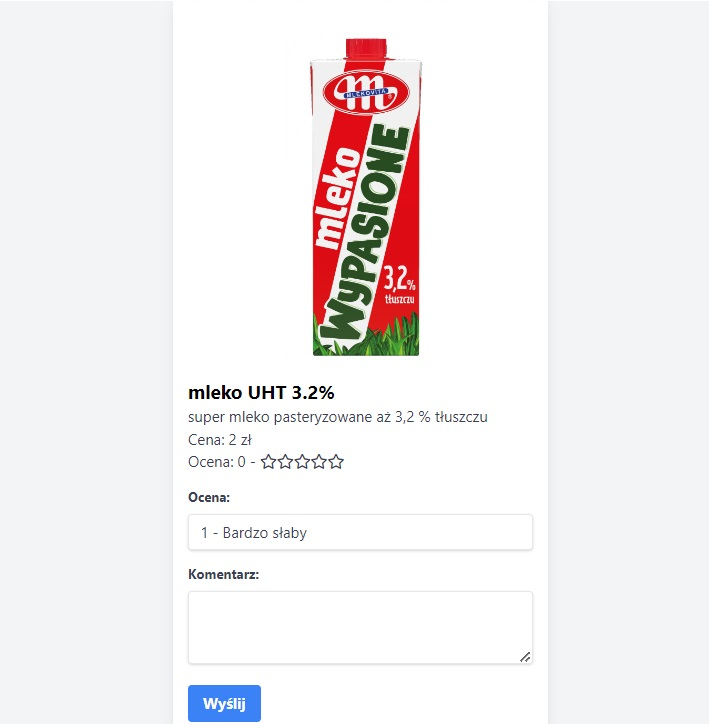
\includegraphics[width=\textwidth]{04paneluzytkownika.jpg}

    
\end{itemize}

\chapter{Opis Technologiczny}
Projekt Megusta wykorzystuje następujące technologie:
\begin{itemize}
    \item \textbf{PHP}: Główny język programowania używany do tworzenia logiki serwera i dynamicznego generowania treści.
    \item \textbf{MySQL}: System zarządzania bazą danych, który przechowuje dane aplikacji, takie jak użytkownicy i treści.
    \item \textbf{Tailwind CSS}: Framework CSS typu utility-first, używany do stylizacji elementów HTML w aplikacji.
    \item \textbf{Composer}: Menedżer zależności PHP, który automatycznie instaluje i zarządza zewnętrznymi bibliotekami i komponentami.
    \item \textbf{Apache}: Serwer webowe używany do hostowania aplikacji.
\end{itemize}

\chapter{Wyszczególnione Wdrożone Zagadnienia Kwalifikacyjne}

Projekt Megusta obejmuje wdrożenie kilku istotnych zagadnień kwalifikacyjnych:
\begin{itemize}
    \item \textbf{Zarządzanie Sesjami i Autoryzacja}: Obsługa sesji użytkowników, w tym logowanie, ciasteczka językowe oraz autoryzacja dostępu do panelu administracyjnego.
    \item \textbf{Bezpieczeństwo Aplikacji}: Zabezpieczenia przed nieautoryzowanym dostępem do panelu administracyjnego oraz sanitacja danych wejściowych do bazy danych w celu zapobiegania atakom SQL injection.
    \item \textbf{Logowanie i Monitorowanie}: Implementacja klasy \texttt{MyLogger} do logowania aktywności użytkowników i błędów systemowych.
    \item \textbf{Dynamiczne Generowanie Treści}: Użycie systemu szablonów i klasy \texttt{HTMLGenerator} do dynamicznego generowania stron na podstawie parametrów URL i danych z bazy.
    \item \textbf{Wielojęzyczność}: Automatyczne wykrywanie preferencji językowych przeglądarki i dostosowywanie treści strony do wybranego języka.
\end{itemize}

\begin{table}[H]
\centering
\begin{tabular}{|c|m{4cm}|m{7cm}|c|}
\hline
\# & Zagadnienie & Opis & Wdrożenie \\
\hline
1 & framework MVC & wykorzystanie frameworka na backendzie & - \\
\hline
2 & framework CSS & wykorzystanie frameworka na frontendzie & + \\
\hline
3 & baza danych & dołączenie do projektu bazy danych & + \\
\hline
4 & cache & dołączenie do projektu systemu cache & - \\
\hline
5 & dependency manager & dołączenie do projektu systemu zarządzania zależnościami & + \\
\hline
6 & HTML & szkielet aplikacji internetowej & + \\
\hline
7 & CSS & ostylowanie aplikacji internetowej & + \\
\hline
8 & JavaScript & uinteraktywnienie aplikacji internetowej & + \\
\hline
9 & routing & wykorzystany routing i tzw. pretty URLs & + \\
\hline
10 & ORM & wykorzystane mapowanie obiektowo-relacyjne & + \\
\hline
11 & uwierzytelnianie & zaimplementowane mechanizmy uwierzytelnienia & + \\
\hline
12 & lokalizacja & możliwość przełączania języka aplikacji & + \\
\hline
13 & mailing & wysyłanie mejli z aplikacji & + \\
\hline
14 & formularze & przesyłanie danych do aplikacji przez formularze & + \\
\hline
15 & asynchroniczne interakcje & zaimplementowane asynchroniczne interkacje z serwerem & + \\
\hline
16 & konsumpcja API & wykorzystanie zewnętrznego API & + \\
\hline
17 & publikacja API & wystawienie własnego API & - \\
\hline
18 & RWD & responsywny frontend & + \\
\hline
19 & logger & logowanie akcji w systemie & + \\
\hline
20 & deployment & wdrożenie aplikacji internetowej & + \\
\hline
\end{tabular}
\label{tab:zagadnienia}
\end{table}



\chapter{Instrukcja Lokalnego i Zdalnego Uruchomienia Systemu}

\section{Lokalna Instalacja}

\subsection{Klonowanie Repozytorium}
Sklonuj repozytorium na lokalny serwer i zainstaluj zależności za pomocą Composer.
\begin{verbatim}
git clone https://github.com/yourusername/megusta.git
cd megusta
composer install
\end{verbatim}

\subsection{Konfiguracja Bazy Danych}
Skonfiguruj połączenie z bazą danych w pliku \texttt{DB.php}.
\begin{verbatim}
$this->db = new mysqli("host", "user", "password", "database");
\end{verbatim}

\subsection{Uruchomienie Serwera}
Skonfiguruj serwer Apache. Przenieś wszyskie pliki do katalogu htdocs. Zaimportuj bazę danych.

\subsection{Odwiedź Stronę}
Otwórz przeglądarkę i przejdź pod adres \texttt{http://localhost/index.php}.

\section{Zdalna Instalacja}

\subsection{Wdrażanie na Serwerze Zdalnym}
Zaloguj się na serwer zdalny i sklonuj repozytorium na serwer. W przypadku korzystania ze środowiska IDE PHP Storm możesz to zrobić poprzez funkcję Deployment. 
\begin{verbatim}
git clone https://github.com/yourusername/megusta.git
cd megusta
composer install
\end{verbatim}

\subsection{Konfiguracja Bazy Danych}
Skonfiguruj połączenie z bazą danych w pliku \texttt{DB.php}.
\begin{verbatim}
$this->db = new mysqli("host", "user", "password", "database");
\end{verbatim}

\subsection{Konfiguracja Serwera Webowego}
Skonfiguruj serwer Apache, aby wskazywał na katalog projektu. Upewnij się, że moduły PHP są włączone (np. \texttt{mod\_php} w Apache).

\subsection{Konfiguracja DNS}
Skonfiguruj DNS, aby domena wskazywała na adres IP serwera zdalnego.

\subsection{Odwiedź Stronę}
Otwórz przeglądarkę i przejdź pod adres \texttt{https://host358482.xce.pl/}.

\chapter{Wnioski Projektowe}
Projekt \textbf{Megusta} jest przykładem aplikacji webowej, która łączy różne technologie i rozwiązania w celu stworzenia funkcjonalnego, responsywnego i bezpiecznego systemu zarządzania treścią. Wdrożenie wielojęzyczności, dynamicznego generowania treści oraz systemu logowania aktywności pozwala na elastyczne zarządzanie treścią i użytkownikami. Stylizacja za pomocą Tailwind CSS zapewnia spójny i estetyczny wygląd interfejsu użytkownika.

\section{Rekomendacje}
\begin{itemize}
    \item Dalsza optymalizacja kodu pod kątem wydajności i bezpieczeństwa. Uwzględnienie w rozwoju proejktu wykorzystania frameworka - Laravel. 
    \item Rozszerzenie funkcjonalności panelu administracyjnego o dodatkowe moduły zarządzania.
    \item Regularne aktualizacje zależności i komponentów w celu zapewnienia zgodności z najnowszymi standardami.
\end{itemize}

\end{document}
